This chapter details the implementation of the automated solution proposed in Chapter \ref{chap:context}. First, an overview of the various components implemented throughout the project is given. Next, the implementation of a deep network capable of automatically extracting annual density bands present in two dimensional data is discussed. The attempts at implementing a network capable of automatically extracting the annual density bands present in three dimensions are also detailed. Then, the implementation of and reasoning behind the custom accuracy metric are discussed. Finally, the techniques used to estimate the calcification rate from the extracted boundaries are described.

\section{Overview}

A system capable of calculating of the calcification rate given only some section of density data requires the implementation of many separate subcomponents. The diagram below provides an overview of these components and outlines the order in which they were implemented and will be discussed.

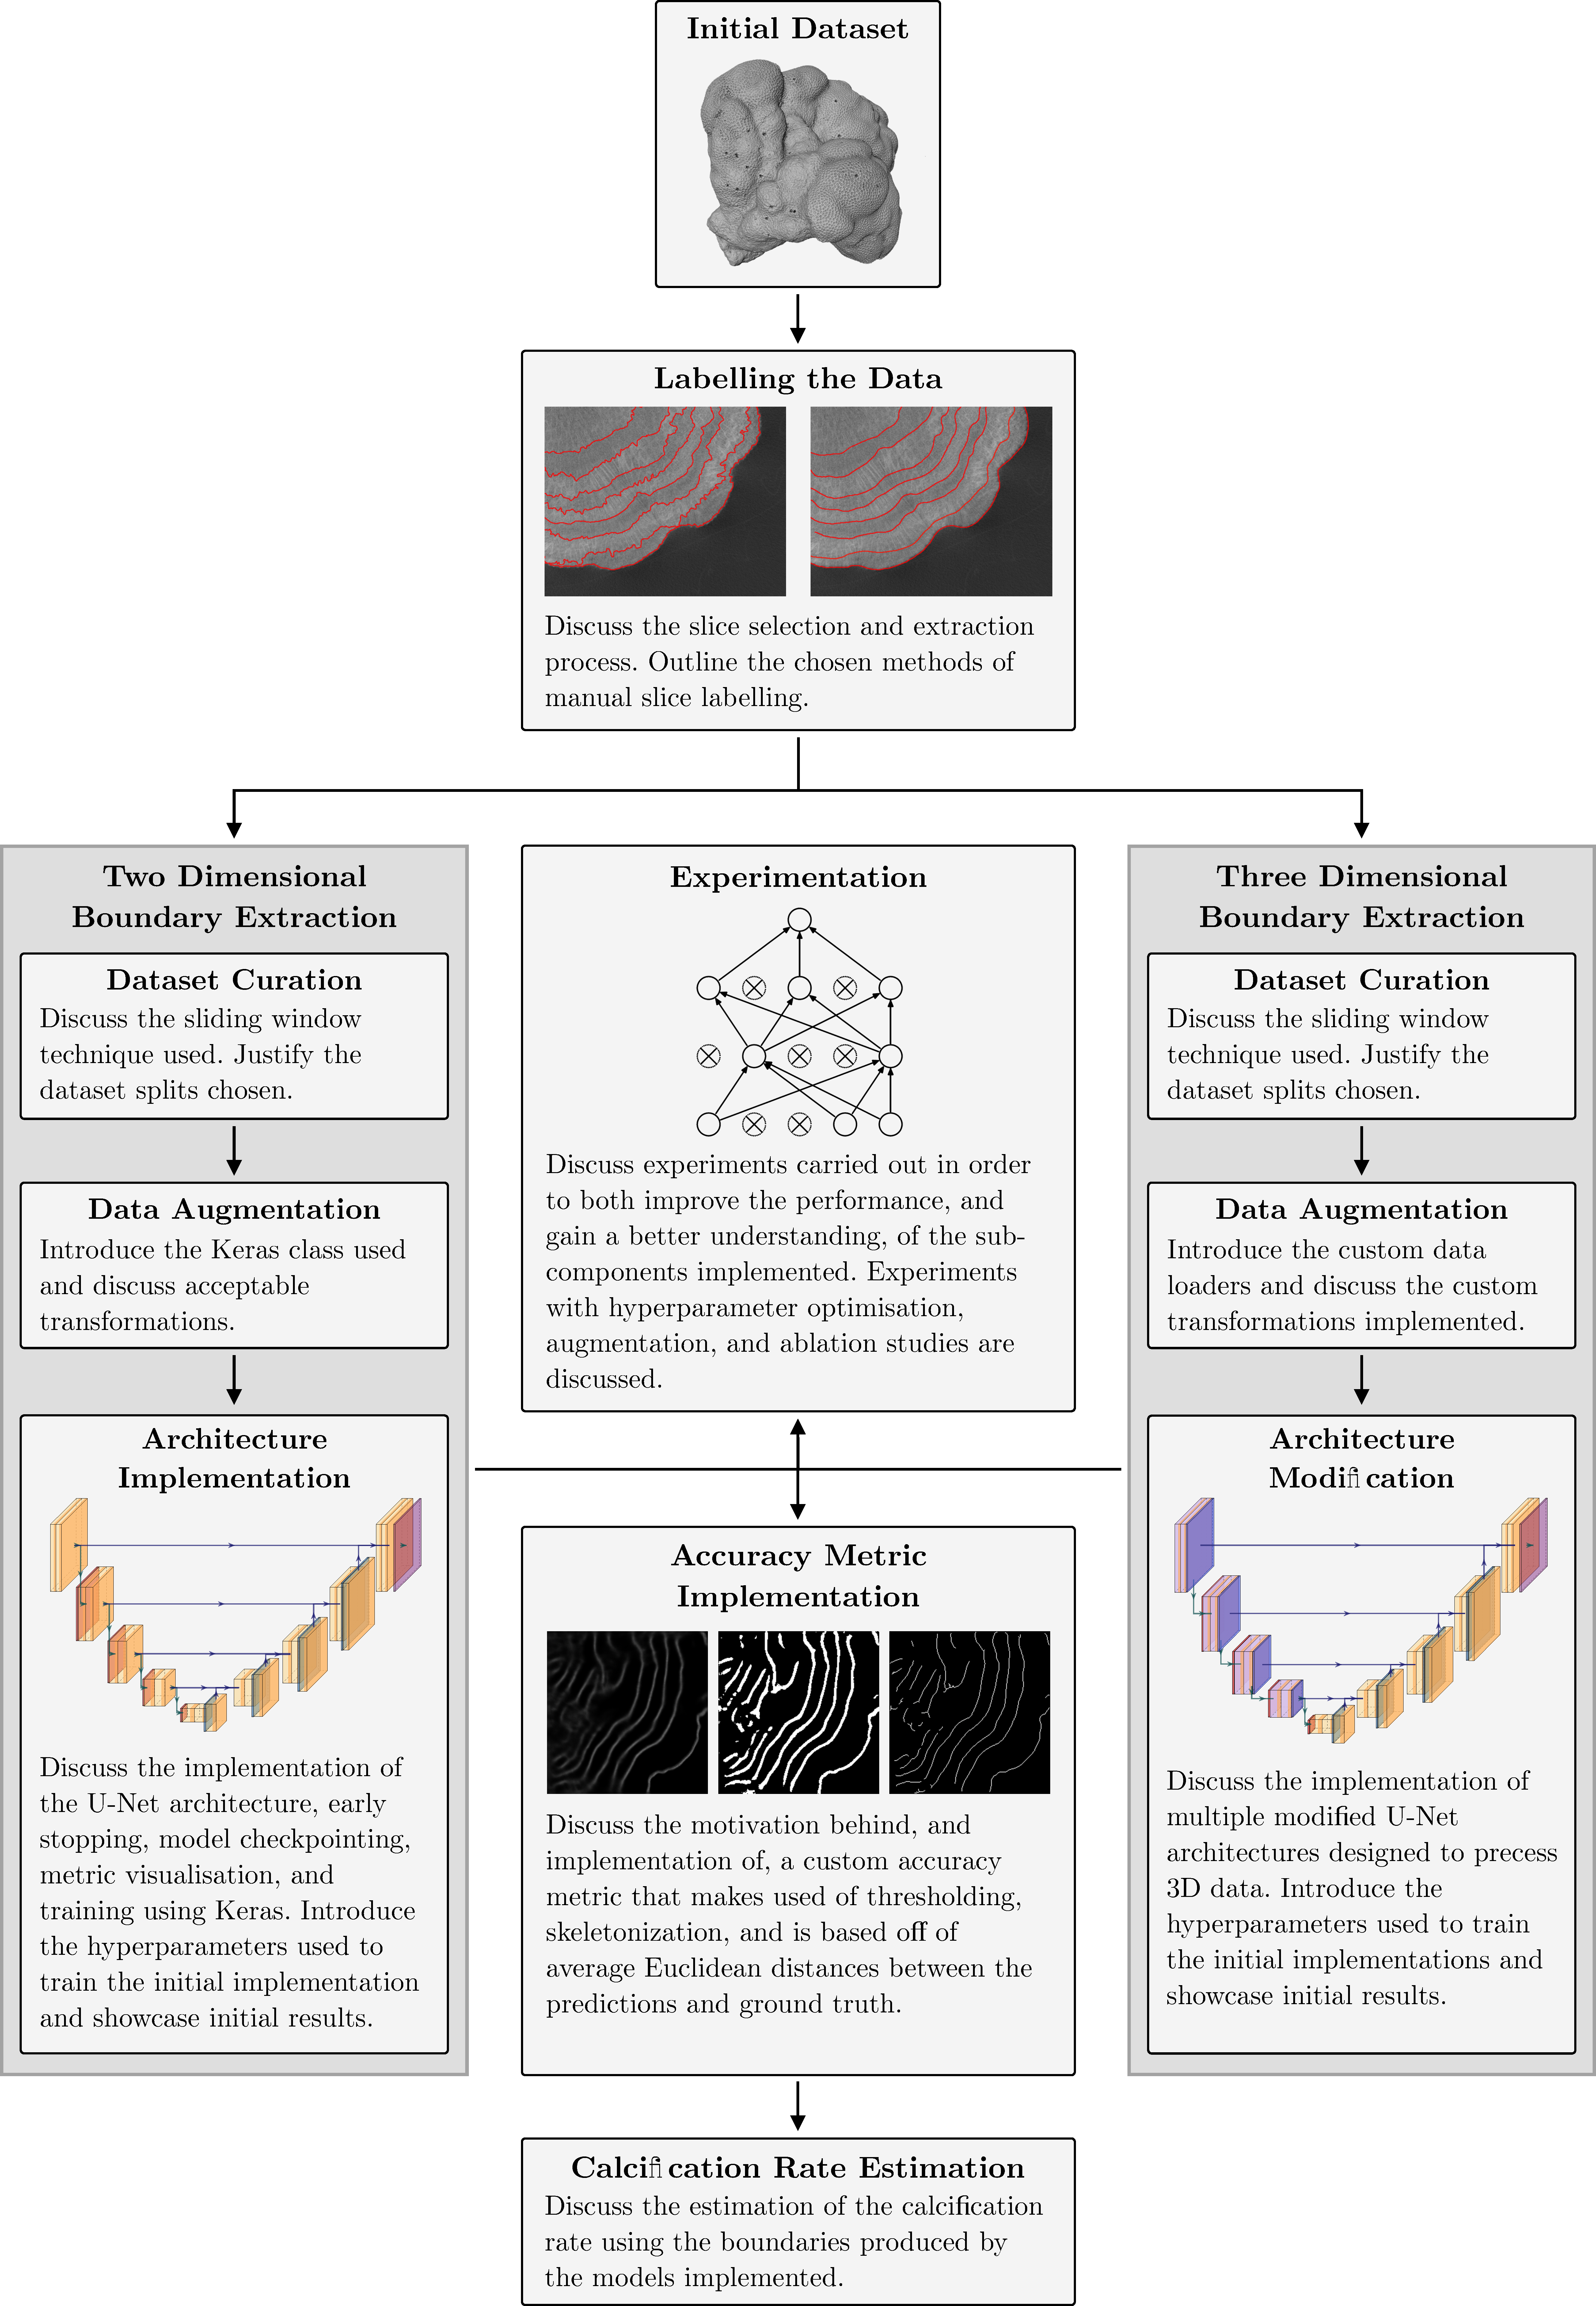
\includegraphics[width=\textwidth, height=0.74\textwidth]{images/overview.pdf}

\section{Two Dimensional Boundary Extraction}

This section outlines the steps taken to implement and train a CNN capable of extracting the annual density banding present in two dimensional data.

\subsection{Labelling the Data}

In order for a supervised CNN to perform well, large amounts of labelled data much be available to train on. Since the dataset provided was initially unlabelled, a manual labelling process was devised and is described in this section.

\subsubsection{The Initial Dataset}

The dataset provided contains more than 160 three dimensional computed tomography (CT) scans of unique coral skeletons from the Natural History Museum's collection. Each individual 3D scan consists of stacks of thousands of 2D \texttt{.tif} images which will be referred to as ``slices''. This unlabelled dataset will be referred to as the ``initial dataset''. Although the initial dataset contains scans of ten different genera of coral, only scans of the Porites genus were considered for labelling and training the network with. An example of a Porites skeleton that is part of the dataset is shown in Figure \ref{fig:scanexample}. The Porites scans were chosen as they contain annual banding that can be more easily identified and labelled.

A typical scan consists of ${\sim}2000$ slices that each have the same resolution of ${\sim}$2000$\times$2000 pixels resulting in an overall 3D resolution of 2000$\times$2000$\times$2000 voxels. The 3D resolution of each scan varies, but the scale (e.g., the number of voxels used to represent a centimetre cubed) is consistent across scans.

\begin{figure}[t]
    \centering
    \begin{subfigure}[t]{0.49\textwidth}
        \centering
        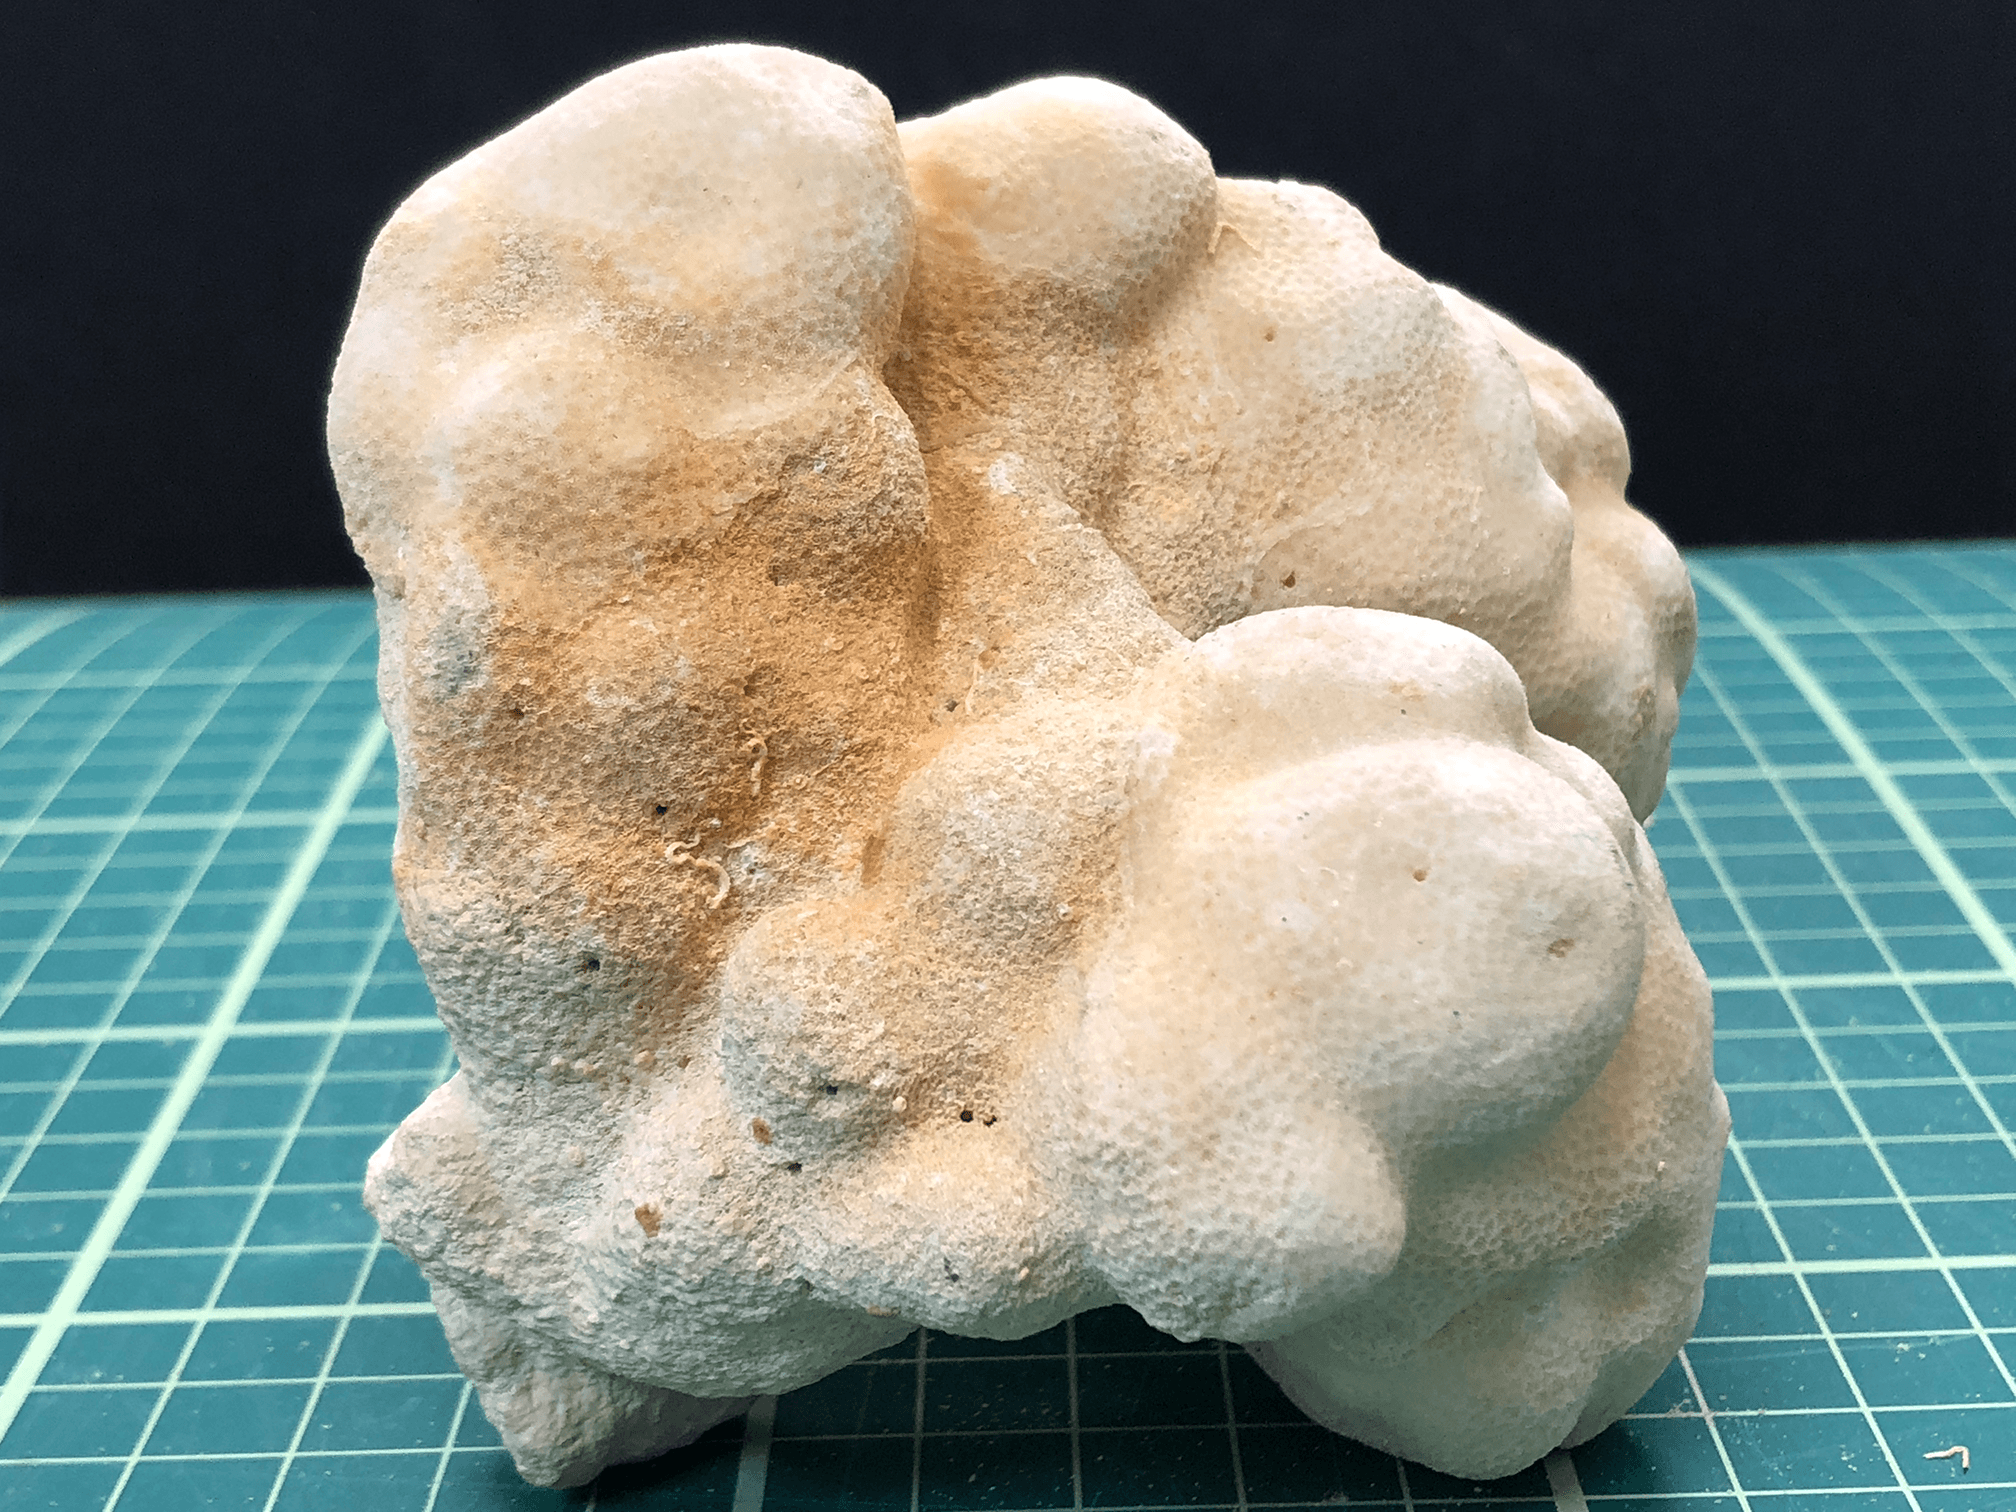
\includegraphics[width=1\textwidth, valign=c]{images/real-coral.png}
    \end{subfigure}
    ~
    \begin{subfigure}[t]{0.49\textwidth}
        \centering
        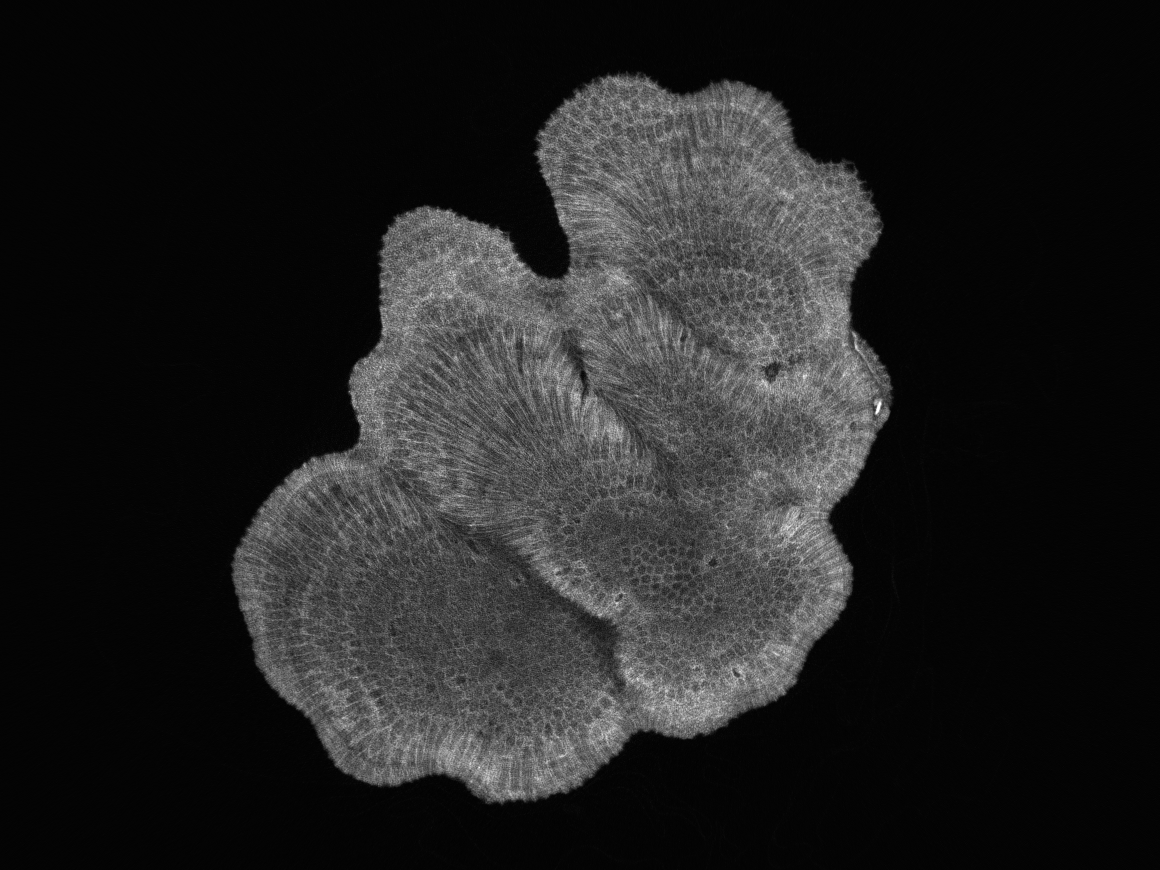
\includegraphics[width=1\textwidth, valign=c]{images/slice-example.png}
    \end{subfigure}
    \caption{\textbf{(left)} An example of a Porites coral skeleton from the Natural History Museum's collection. This particular sample was collected from the Solomon Islands in 1974. In the initial dataset, the scan of this sample is represented by 1945$\times$1508$\times$1208 voxels. \textbf{(right)} A 2D slice extracted from the CT scan of the sample shown on the left. The slice is a negative; brighter pixels correspond to high density and darker pixels correspond to low density.}
    \label{fig:scanexample}
\end{figure}

\subsubsection{Slice Selection and Extraction}

Not all slices that compose a scan contain annual density banding that can confidently be identified. In order to find appropriate slices, each Porites scan was opened and inspected manually using a 3D visualisation program called Avizo\footnote{\url{https://tiny.cc/avizo}}. Avizo allows users to view slices orthogonal to the $x$, $y$, or $z$ axis of a scan. A selection of six slices that could confidently be labelled were chosen. MAYBE HAVE A SENTENCE HERE EXPLAINING THAT THE BEST SLICES ARE OFTEN ORTHOGONAL TO THE GROWTH DIRECTION AND SO ARE ROUGHLY HALFWAY THRU THE SCAN? Once these slices were identified, a Python script was used to extract each slice and export them as greyscale PNG images. The slices can be represented as greyscale images since they only require one channel to represent depth. Some of the adjacent slices were also extracted in order to curate the 3D dataset used later in the project (discussed in Section~\ref{sec:threedimension}).

\subsubsection{Slice Labelling}

Once the slices were selected, a labelling process was established. Initially, two methods of labelling were considered and shown to Dr Erica Hendy, a senior lecturer in biogeochemical cycles. Of the two methods (shown in Figure \ref{fig:labelstyle}), the ``smooth'' method was deemed as the more realistic choice. An idealised annual density cycle is actually in the form of a sinusoidal wave with the density gradually changing from high to low and back over the course of a year~\cite[p. 39]{coralsine}. Thus, an exact boundary between a high and low band does not actually exist, making the ``complex'' method unrealistic both in terms of reproducibility, and in terms of biological accuracy.

\begin{figure}[t]
    \centering
    \begin{subfigure}[t]{0.49\textwidth}
        \centering
        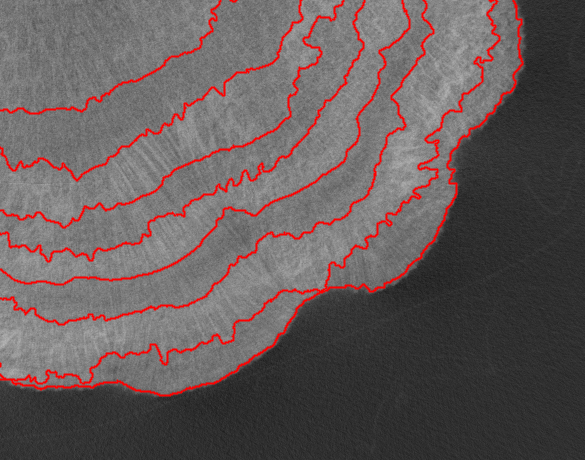
\includegraphics[width=1\textwidth, valign=c]{images/rough-label.png}
    \end{subfigure}
    ~
    \begin{subfigure}[t]{0.49\textwidth}
        \centering
        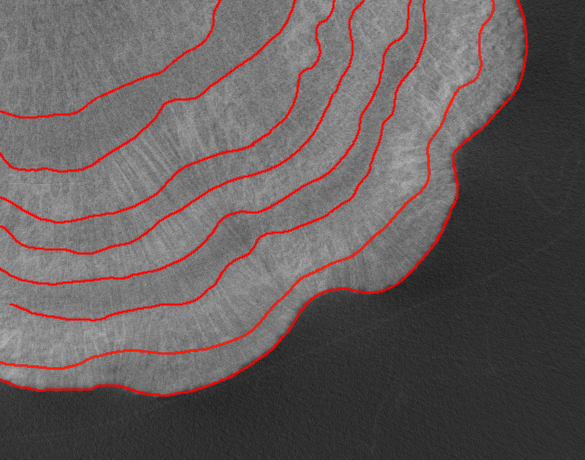
\includegraphics[width=1\textwidth, valign=c]{images/smooth-label.png}
    \end{subfigure}
    \caption{A comparison of the two methods of labelling that were initially considered. The boundary labels are coloured red and placed over the the same original negative 2D slice. \textbf{(left)} A method of labelling in which the boundaries were placed at the sharpest change in density resulting in complex boundaries whose positions are highly sensitive to noise in the image. \textbf{(right)} A method in which the chosen boundaries are ``smooth'' whilst also being placed as close as possible to the sharpest changes in density.}
    \label{fig:labelstyle}
\end{figure}

Each selected slice was then manually labelled using the GNU Image Manipulation Program (GIMP)\footnote{\url{https://www.gimp.org}}. A one pixel wide white line is drawn at the beginning and end of each annual high density band and the rest of the image is black---no values other than black or white are present in the labels. In order to ensure that the decisions made regarding the boundaries of the annual bands were as consistent as possible, each slice was manually labelled three or more times, and the most common boundaries were chosen. It is important for the labelling method to be consistent and reproducible as this enables the dataset to be expanded in the future.

\subsection{Dataset Curation}

With only a small selection of slices successfully extracted and labelled, a larger dataset of image-label pairs was required for the model to train on.

\subsubsection{Sliding Window}

In order to expand the dataset, a sliding window technique was used. A script was written in Python that took a slice, two 2D coordinates, a ``stride'', and a size as arguments. The pair of coordinates corresponded to the top left corner and bottom right corner of the confidently labelled area of the slice. This was the area that the window would slide over in order to create the resulting ``patches''. The stride argument dictated how far the window should slide before each patch was produced. The most common stride value used was 20. The size argument defined how large to resulting patches should be. The patches initially produced had a resolution of 256$\times$256 pixels, but various sizes of patches were experimented with and are discussed in Chapter \ref{chap:evaluation}. The arguments used in order to produce the curated dataset used in this project are shown in Table \ref{tab:slidingwindow}. A total of 388 patches were produced from six slices taken from four different coral skeletons. This dataset of 388 256$\times$256 patches and their corresponding labels were stored as greyscale \texttt{.png} images.

\begin{table}[t]
\centering
\caption{A table showing the arguments used with the Python script for each labelled slice. For each slice, a size argument of 256 was also specified. Note that some slices are represented by two rows as these slices contained two separate areas that could be confidently labelled. It was not possible to use one area that contains the two areas as this would result in multiple patches with no labelling being produced.}
\begin{tabular}{@{}lrrrrrr@{}}
\toprule
Slice & $x_{top}$ & $y_{top}$ & $x_{bottom}$ & $y_{bottom}$ & Stride (px) & Patches produced \\ \midrule
RS0030\_yz\_0625.tif    & 1028      & 153       & 1350         & 530          & 20          & 36      \\
RS0030\_yz\_0642.tif    & 1070      & 143       & 1390         & 463          & 20          & 18      \\
RS0030\_yz\_0642.tif    & 895       & 400       & 1275         & 685          & 20          & 12      \\
RS0116\_0414.tif        & 666       & 1258      & 1560         & 1750         & 40          & 150     \\
RS0116\_0500.tif        & 970       & 1320      & 1320         & 1854         & 30          & 54      \\
RS0116\_0500.tif        & 1130      & 1250      & 1525         & 1730         & 30          & 56      \\
RS0128\_yz\_0451.tif    & 490       & 258       & 790          & 690          & 20          & 32      \\
RS0130\_xz\_0820.tif    & 513       & 1190      & 828          & 1485         & 10          & 30      \\ \midrule
Total                   &           &           &              &              &             & 388     \\ \bottomrule
\end{tabular}
\label{tab:slidingwindow}
\end{table}

In order to prevent the dataset from representing certain coral samples better than others, an effort was made to equalise the number of patches produced per scan. Due to different slices containing varying sizes of confidently labelled areas, the stride argument was used to increase or reduce the number of patches produced. However, it was also important to produce as much data as possible to enable the network to perform well. Ultimately, some slices produced almost five times as many slices as others resulting in some imbalance in the types of coral scans represented by the dataset. Although this could negatively affect the generalisability of a network trained on this dataset, cross-validation with carefully selected splits to represent each coral scan was ultimately used and is discussed in Section \ref{sec:evalcrossval}.

\subsubsection{Splitting the Dataset}

For the initial training and testing of the network, the curated dataset was split into a training set, a validation set, and a test set. Of the 388 patches, 322 were used for training, 56 for testing, and 10 for validation. The patches composing the test and validation sets were all produced from slices of a coral skeleton that was not part of the training set. This ensured that the network could not have been overfitting to the nature of the annual banding present in the skeleton used for testing. If this had been the case, the performance on the test data could have been positively skewed.

\subsection{Data Augmentation}

As discussed in Section \ref{sec:regularization}, data augmentation is an important regularization technique. Since only 388 patches had been produced, extensive augmentation was used to artificially expand the dataset. This data augmentation later proved effective in improving the performance achieved by the network and is discussed further in Section \ref{sec:evalaugmentation}.

\subsubsection{The Keras \texttt{ImageDataGenerator} class}

The Keras library allows users easily implement augmentation using the \texttt{ImageDataGenerator} class\footnote{\url{https://keras.io/preprocessing/image}}. In this case, the \texttt{flow\_from\_directory} method was used to perform online augmentation. This method first loads images from a directory into batches. A series of random transformations are then applied to each batch before replacing the original batches with these new randomly transformed batches. A network trained on the generator produced by this method will therefore be trained on randomly transformed samples as opposed to the original samples themselves.

\begin{lstlisting}[float={t},caption={A simplified example of online augmentation implemented using the \texttt{ImageDataGenerator} class. The model is then trained for five epochs with each epoch consisting of 1000 training samples.},label={lst:augment},language=Python,upquote=true]
from keras.preprocessing.image import ImageDataGenerator
import random

# Specify the transformations allowed and store them in a dictionary
aug = dict(rotation_range=2,
           width_shift_range=0.02,
           height_shift_range=0.02,
           shear_range=2,
           zoom_range=0.02,
           brightness_range=[0.9,1.1],
           horizontal_flip=True,
           vertical_flip=True,
           fill_mode="nearest")

# Pass the contents of the dictionary as arguments to the ImageDataGenerator
# constructors
image_datagen = ImageDataGenerator(**aug)
label_datagen = ImageDataGenerator(**aug)

# Generate a random seed to be used for both the image and label generators
seed = random.randint(0, 100)

# Create the generators using the flow_from_directory method. The same seed
# value is passed to both methods ensuring the same transformations are applied.
image_generator = image_datagen.flow_from_directory(image_path, seed=seed, ...)
label_generator = label_datagen.flow_from_directory(label_path, seed=seed, ...)

# Zip the generators into one generator that yields image-label pairs
train_generator = zip(image_generator, label_generator)

# Fit the model using the zipped generator
model.fit_generator(train_generator, steps_per_epoch=1000, epochs=5, ...)
\end{lstlisting}
Since the \texttt{flow\_from\_directory} method applies random transformations to each image, the random transformations must also be applied to the corresponding labels. This can be achieved by passing the same value to the \texttt{seed} argument of the \texttt{flow\_from\_directory} methods used to load the images and labels. This method is also capable of shuffling the order in which images are loaded and trained with. Using the same seed value also ensures that this shuffling follows the same order for both the images and labels. The actual transformations to be used when augmenting the data are specified using various arguments passed to the \texttt{ImageDataGenerator} constructor. A simplified example demonstrating the implementation of the training generator and the transformations used is shown in Listing \ref{lst:augment}.

Since the training generator will yield randomly augmented image-label pairs indefinitely, the \texttt{steps\-per-epoch} argument defines how many samples should be processed before an epoch is considered complete.

\subsubsection{Acceptable Augmentations}

The possible transformations specified each have a random chance of being applied to each image. It was important to choose a range of possible transformations that would always produce a reasonable augmented image. The permitted augmentations that could be randomly chosen were:

\begin{itemize}
    \item Rotations within a range of $\pm 2$ degrees.
    \item Shifts in the $x$ axis within a range of $\pm 2\%$ of the images' widths.
    \item Shifts in the $y$ axis within a range of $\pm 2\%$ of the images' heights.
    \item Shears within a range of $\pm 2$ degrees.
    \item Zooms in the $x$ and $y$ axes within a range of $\pm 2\%$ of the images' widths or heights.
    \item Brightness shifts within a range of $\pm 10\%$.
    \item Horizontal flips and vertical flips.
\end{itemize}

Using larger ranges of permitted transformations resulted in augmented images that did not represent the real data well. Examples of images created using the ranges defined above and images created using ``unrealistic'' ranges are shown in Figure \ref{fig:augexample}.

\begin{figure}[t]
    \centering
    \begin{subfigure}[t]{0.18\textwidth}
        \centering
        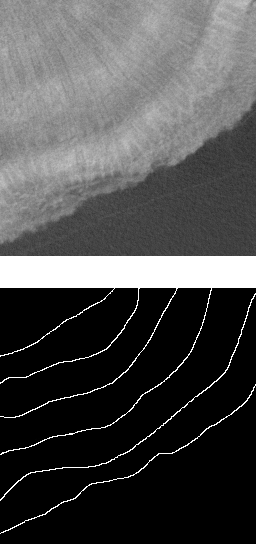
\includegraphics[width=1\textwidth, valign=c]{images/orig-aug.png}
        \caption{Original}
    \end{subfigure}
    ~
    \begin{subfigure}[t]{0.38\textwidth}
        \centering
        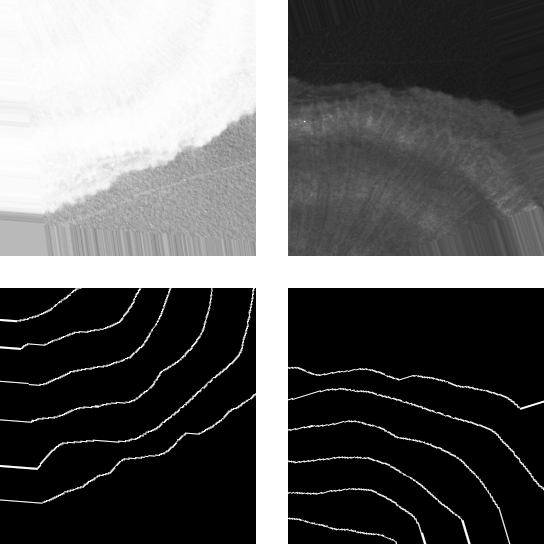
\includegraphics[width=1\textwidth, valign=c]{images/bad-aug.png}
        \caption{Unrealistic}
    \end{subfigure}
    ~
    \begin{subfigure}[t]{0.38\textwidth}
        \centering
        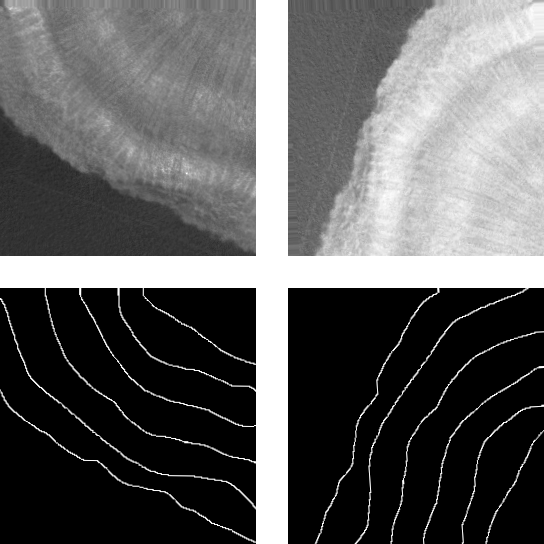
\includegraphics[width=1\textwidth, valign=c]{images/good-aug.png}
        \caption{Realistic}
    \end{subfigure}
    \caption{Examples of augmented images created using both ``realistic'' and ``unrealistic'' sets of permitted transformations. The images are shown at the top and their corresponding labels are shown at the bottom. All labels are thresholded after augmentation to ensure that only white or black values are present. \textbf{(a)} The original image-label pair. \textbf{(b)} Two examples of image-label pairs augmented using a set of unrealistic permitted transformations resulting in images that do not represent the real coral data well. The first image's brightness has been shifted too far. The overly aggressive rotation has resulted in straight labels on the left-most edge which are not realistic. The second image's label has also been rotated too far resulting in a straight label on the right-most edge. \textbf{(c)} Two examples of image-label pairs augmented using the set of permitted transformations used in this project.}
    \label{fig:augexample}
\end{figure}

\subsection{U-Net}

As discussed in Chapter \ref{chap:technical}, the U-Net architecture~\cite{ronneberger2015u} is the main architecture experimented with. The implementation used throughout the project was initially based off of an implementation available on GitHub\footnote{\url{https://github.com/zhixuhao/unet}}, though over the course of the project the majority of the code was edited. It is written in Python and makes use of the Keras functional API.

Recall that the original U-Net architecture consists of three sections: the contracting path, the bottleneck, and the expanding path. The contracting path consists of multiple ``blocks'' with each block consisting of two convolutional layers each using 3$\times$3 kernels and the ReLU activation function followed by a 2$\times$2 max-pooling layer using a stride of 2. After the first contracting block, each successive block doubles the number of feature channels. The first contracting block is implemented like so:
\begin{lstlisting}[language=Python,upquote=true,belowskip=0pt]
conv1 = Conv2D(64, 3, activation="relu", padding="same")(inputs)
conv1 = Conv2D(64, 3, activation="relu", padding="same")(conv1)
pool1 = MaxPooling2D(pool_size=(2, 2))(conv1)
\end{lstlisting}
The \texttt{pool1} tensor will be the input to the next contracting block, and so on. The first argument of the \texttt{Conv2D} function is the number of output feature channels. Since the number of feature channels doubles at each contracting block, the next contracting block would have 128 feature channels rather than 64. The second argument is the size of the convolution kernels to use, so 3$\times$3 in this case. The padding argument specifies that the dimensions of the output feature channels should match the dimensions of the inputs. This differs from the implementation of the U-Net architecture used in the original paper and will be explained later in this section. The Keras \texttt{MaxPooling2D} function implicitly uses the same stride size as the pool size specified, so a stride of two in the $x$ and $y$ axes will be used.

The bottleneck contains only one block. This block also consists of two convolutional layers each using 3$\times$3 kernels and the ReLU activation function, but no max-pooling layers are present. Thus, the bottleneck block is implemented similarly to the block shown above, only without the max-pooling layer. Note that at this point, the number of output feature channels has reached 1024.

The expanding path consists of multiple blocks with each block containing an up

\begin{lstlisting}[language=Python,upquote=true,belowskip=0pt]
up9 = UpSampling2D(size=(2, 2))(conv8)
up9 = Conv2D(64, 2, activation="relu", padding="same")(up9)
merge9 = concatenate([conv1, up9], axis=3)
conv9 = Conv2D(64, 3, activation="relu", padding="same")(merge9)
conv9 = Conv2D(64, 3, activation="relu", padding="same")(conv9)
\end{lstlisting}

Every  step  in  the  expansive  path  consists  of  an  upsampling  of  thefeature map followed by a 2x2 convolution (“up-convolution”) that halves thenumber of feature channels, a concatenation with the correspondingly croppedfeature  map  from  the  contracting  path,  and  two  3x3  convolutions,  each  fol-lowed by a ReLU.

How it differs from original unet:
- padding is 'same' rather than none. Allows reconstruction back to exactly the same size? Is this possible in original paper?
- the point above means that we no longer need to crop before we concatenate.
- upsampling rather than upconvolutions?

Implementation of a block

Spatial drop out better for fully conv? \url{https://arxiv.org/pdf/1411.4280.pdf}

% From Keras docs I think
% This version performs the same function as Dropout, however it drops
% entire 2D feature maps instead of individual elements. If adjacent pixels
% within feature maps are strongly correlated (as is normally the case in
% early convolution layers) then regular dropout will not regularize the
% activations and will otherwise just result in an effective learning rate
% decrease. In this case, SpatialDropout2D will help promote independence
% between feature maps and should be used instead.

\subsection{SegNet}

\subsection{Training}

\subsubsection{Early Stopping and Checkpointing}

\section{Three Dimensional Boundary Extraction}
\label{sec:threedimension}

This section discusses the attempts to implement and train a CNN capable of extracting the annual density banding present in three dimensional data.

\subsection{Dataset Expansion}

\subsection{Data Loader Implementation}

\subsection{Three Dimensional Data Augmentation}

\subsection{Architecture Modification}

\section{Accuracy Metric Implementation}

\subsection{Skeletonisation}

(Show algorithm and maybe some source code?)

\subsection{The \texttt{ctypes} Module}

\section{Density Band Width Estimation}

\subsection{Point Sampling}

% {\bf A topic-specific chapter, of roughly $15$ pages} 
% \vspace{1cm} 

% \noindent
% This chapter is intended to describe what you did: the goal is to explain
% the main activity or activities, of any type, which constituted your work 
% during the project.  The content is highly topic-specific, but for many 
% projects it will make sense to split the chapter into two sections: one 
% will discuss the design of something (e.g., some hardware or software, or 
% an algorithm, or experiment), including any rationale or decisions made, 
% and the other will discuss how this design was realised via some form of 
% implementation.  

% This is, of course, far from ideal for {\em many} project topics.  Some
% situations which clearly require a different approach include:

% \begin{itemize}
% \item In a project where asymptotic analysis of some algorithm is the goal,
%       there is no real ``design and implementation'' in a traditional sense
%       even though the activity of analysis is clearly within the remit of
%       this chapter.
% \item In a project where analysis of some results is as major, or a more
%       major goal than the implementation that produced them, it might be
%       sensible to merge this chapter with the next one: the main activity 
%       is such that discussion of the results cannot be viewed separately.
% \end{itemize}

% \noindent
% Note that it is common to include evidence of ``best practice'' project 
% management (e.g., use of version control, choice of programming language 
% and so on).  Rather than simply a rote list, make sure any such content 
% is useful and/or informative in some way: for example, if there was a 
% decision to be made then explain the trade-offs and implications 
% involved.

% \section{Example Section}

% This is an example section; 
% the following content is auto-generated dummy text.
% \lipsum

% \subsection{Example Sub-section}

% \begin{figure}[t]
% \centering
% foo
% \caption{This is an example figure.}
% \label{fig}
% \end{figure}

% \begin{table}[t]
% \centering
% \begin{tabular}{|cc|c|}
% \hline
% foo      & bar      & baz      \\
% \hline
% $0     $ & $0     $ & $0     $ \\
% $1     $ & $1     $ & $1     $ \\
% $\vdots$ & $\vdots$ & $\vdots$ \\
% $9     $ & $9     $ & $9     $ \\
% \hline
% \end{tabular}
% \caption{This is an example table.}
% \label{tab}
% \end{table}

% \begin{algorithm}[t]
% \For{$i=0$ {\bf upto} $n$}{
%   $t_i \leftarrow 0$\;
% }
% \caption{This is an example algorithm.}
% \label{alg}
% \end{algorithm}

% \begin{lstlisting}[float={t},caption={This is an example listing.},label={lst},language=C]
% for( i = 0; i < n; i++ ) {
%   t[ i ] = 0;
% }
% \end{lstlisting}

% This is an example sub-section;
% the following content is auto-generated dummy text.
% Notice the examples in Figure~\ref{fig}, Table~\ref{tab}, Algorithm~\ref{alg}
% and Listing~\ref{lst}.
% \lipsum

% \subsubsection{Example Sub-sub-section}

% This is an example sub-sub-section;
% the following content is auto-generated dummy text.
% \lipsum

% \paragraph{Example paragraph.}

% This is an example paragraph; note the trailing full-stop in the title,
% which is intended to ensure it does not run into the text.
